\section[Rumtime object in memory]{运行时数据模型}
本节\href{http://www.programcreek.com/2011/11/what-do-java-objects-look-like-in-memory/}{参考网址}。

\subsection[Fields in memory]{Fields in memory}
运行时期,对象在内存中的样子大致如图\ref{fig:base}所示。
\begin{figure}
  \centering
  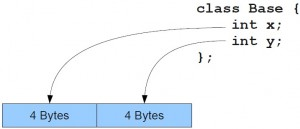
\includegraphics[width=0.8\textwidth]{picturedir/base.jpg}\\
  \caption{Runtime object in Heap}\label{fig:base}
\end{figure}

存在继承关系时的情形如图\ref{fig:derived}所示。
\begin{figure}
  \centering
  % Requires \usepackage{graphicx}
  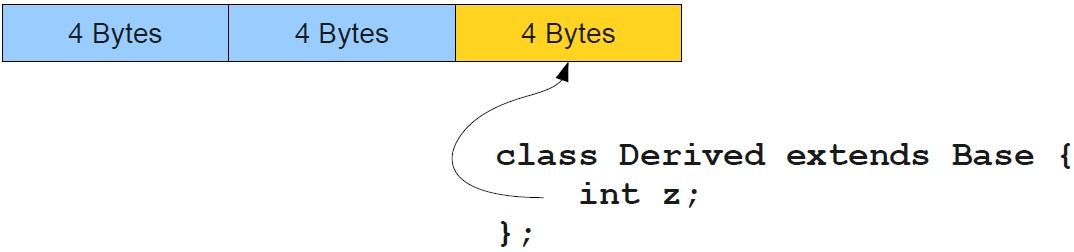
\includegraphics[width=0.8\textwidth]{picturedir/derived.jpg}\\
  \caption{Objects of Hierachy in Heap}\label{fig:derived}
\end{figure}

\subsection[Methods in memory]{Methods in memory}
类似于属性在内存中的布局,方法也可以同样布局,如图\ref{fig:novtable}所示。
\begin{figure}
  \centering
  % Requires \usepackage{graphicx}
  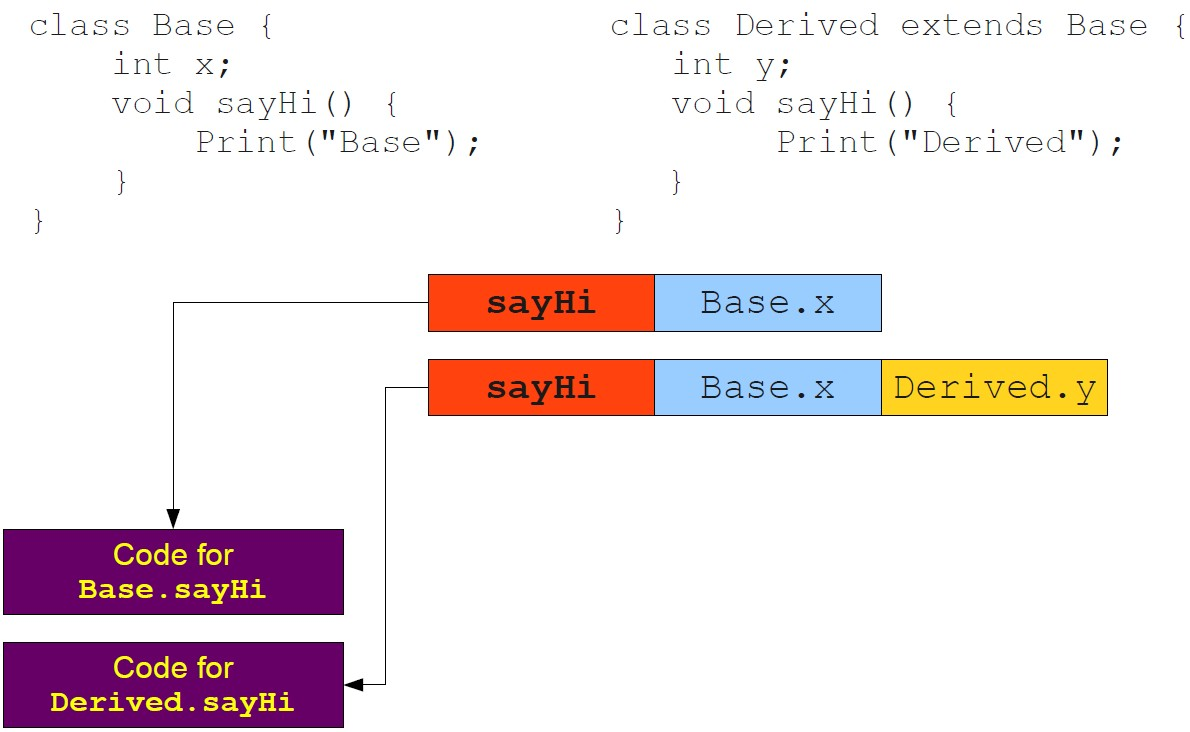
\includegraphics[width=0.8\textwidth]{picturedir/functions-without-vtable.jpg}\\
  \caption{Objects in Heap without VTable}\label{fig:novtable}
\end{figure}
可是,这样一来每个对象都有一堆重复的method pointer,占空大,效率低,不划算,
改进一下,每个类增加一个函数表,而每个对象只需一个指向该函数表的指针即可,
如图\ref{fig:vtable}所示,注意父类、子类有覆盖(override)关系的函数在函数表中
的位置必须是一样的,详见第\ref{sec:dynamicbinding}节。
\begin{figure}
  \centering
  % Requires \usepackage{graphicx}
  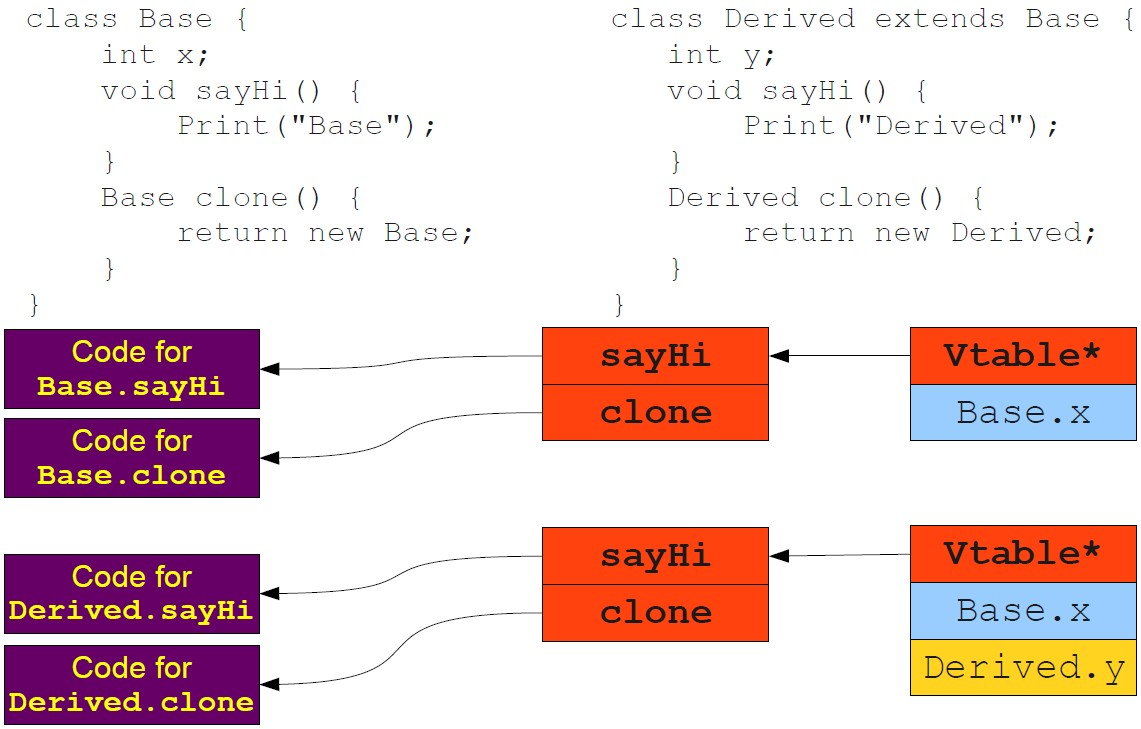
\includegraphics[width=.8\textwidth]{picturedir/objects-in-memory-optimization.jpg}\\
  \caption{Object layout with VTable}\label{fig:vtable}
\end{figure}
